\documentclass{sig-alternate}
\usepackage{times}
\usepackage{epsfig}
\usepackage{graphicx}
\usepackage{amsmath}
\usepackage{amssymb}
\usepackage[breaklinks=true,bookmarks=false]{hyperref}

\begin{document}

\title{Human Activity Recognition with Mobile Sensors}

\author{
Fridtjof Melle\\
Carnegie Mellon University\\
{\tt fmelle@andrew.cmu.edu}
}

\maketitle

%%%%%%%%% ABSTRACT
\begin{abstract}
   With the growing accessibility of accelerometers and movement measurement in our everyday lives largely introduced by smart phones we carry with us to all places the various ways of application are endless. A first step in making this an profitable tool for everyday use is to convert the measurements into something intelligent. Activity Recognition is a rising field where we seek to translate chains of time-series data provided by mobile sensors into specific activities. By intelligently analyzing this data this study seeks to determine what kind of activities are easily or more difficultly recognized using a simple and widely implemented posterior probability measuring classification algorithm.
   
\end{abstract}

%%%%%%%%% BODY TEXT
\section{Introduction}

\subsection{The Problem}
In the growing field of \textit{Human Activity Recognition} we find ourselves surrounded with the complex task of successfully and effectively translating endless variations of time-series recorded sensor data into meaningful resources. While we today profit from a large array of applications that to some extent recognizes human activity, most devices  limit themselves to certain specific types of activities in a given context such as sports or specific tasks. There is still a lot of work left to develop an all-understanding intelligence that can comprehend every type of activity induced into sensible information.

\subsection{The Solution}
In order to address this massive challenge, this research focuses on analyzing what kind of activities that are recognized most effectively, and what kind of activities require more consideration.

Through a simple standardization of an established and widely used dataset for \textit{Human Activity Recognition}, the study seeks to analyze the per-activity performance using the simplest and perhaps most widely used posterior probability classification method by looking at the various improvements that can be amended to it.

%=====================================================================

\section{Background}

\subsection{Dataset}
For the purpose of researching the proposed problem most efficiently, a well-tested and widely researched dataset was taken into consideration. The Skoda Mini Checkpoint dataset was originally created to investigate the use of ensemble classifiers in activity recognition and has been widely implemented over the past years\cite{Zappi08}. 

The dataset contains time-series data from a total of 10 USB sensor accelerometers equally placed and separately recorded on each arm over three hours resulting in about 700,000 data points each representing 33 ms visualized in Figure~\ref{fig:body_sensors}. Every sensor measures over three dimensions simultaneously collecting the effects of a total 10 manipulative gestures performed in a car maintenance scenario, as well as one null activity for reference. The resulting two fully labeled datasets for left and right arm form the basis for our study. 

\begin{figure}
\begin{center}
  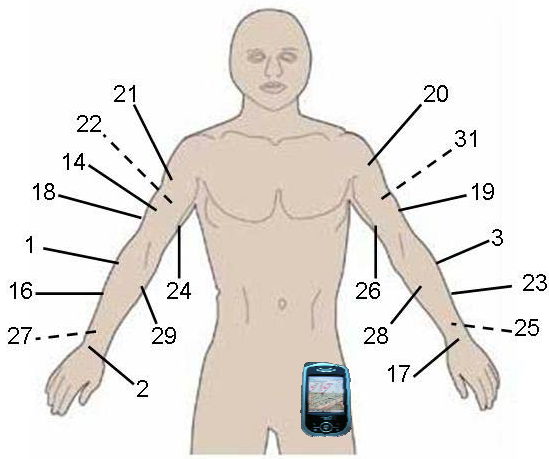
\includegraphics[width=0.6\linewidth]{non_tech_imgs/Body_Sensors.png}
\end{center}
  \caption{Visualization of the mobile sensors placement.}
  \label{fig:body_sensors}
\end{figure}

\begin{table}[bp]
\centering
\caption{Mapping of activities to label values.}
\begin{tabular}{|l|l|}
\hline
\text{Activity}          				&\textbf{Label value} 	\\ \hline
\textbf{Null activity}  				& 32 		 			\\ \hline
\textbf{Write on notepad}	 			& 48		 			\\ \hline
\textbf{Open hood}  					& 49 					\\ \hline
\textbf{Close hood}				 		& 50 					\\ \hline
\textbf{Check Gaps on the front door} 	& 51 					\\ \hline
\textbf{Open left front door}	 		& 52 					\\ \hline
\textbf{Close left front door}			& 53 					\\ \hline
\textbf{Close both left doors}			& 54 					\\ \hline
\textbf{Check trunk gaps}				& 55 					\\ \hline
\textbf{Open and close trunk}			& 56 					\\ \hline
\textbf{Check steering wheel}			& 57 					\\ \hline
\end{tabular}
\label{tab:label_value}
\end{table}

\subsection{Sliding windows and Feature Extraction}
Classifying \textit{Human Activity Recognition} data is effectively translating time-series signal data into specifically performed sequences of gestures forming an activity.

The first step in establishing a dataset that can be injected into a statistical classifier is to evaluate the time-series data delicately. Inspired by previous approaches, an approach to capture local information for primitive-based AR by sliding windows with overflow was decided upon\cite{Huynh}.

With this configuration of the sliding windows, the feature vectors will be assembled by intelligently chosen features as established by previous approaches\cite{Zeng}.

%=====================================================================

\section{Overview}
The study is effectively divided into several main parts, each providing intelligent results towards the issue in question.

\subsection{Baseline Classification Performance}
In a first time we look closer at the baseline performance of our algorithm once applied most elegantly towards a preprocessed version of the original dataset. This approach serves in providing a ground understanding of how well the simplest evaluation of time-series data performs on a very specific set of a limited number of activities once trained on several repetitions of every activity.

\subsection{Combining The Data}
The original data provided by \textit{Skoda Mini Checkpoint} does as mentioned contain data separately measured from sensors equally spread and placed on both arms. While it is interesting to evaluate how various activities are recognized with different amounts of success by each arm individually, the study investigates how intelligently merging the two separate datasets improves the recognition. 

This will consequently provide understanding of how more doubling the amount of information or sensors for each measurement increases the general classification performance.

\subsection{Feature Selection}
When attempting to recognize various activities, different sensors have varying impact on different activities. In collaboration with another team working on the same dataset for \textit{Human Activity Recognition}, the research was enhanced by the possibility of measuring the effect of performing a more extensive feature selection with subsequent dimensionality reduction on the same set of data. 

Looking at the performance of this approach explores the space of improvement in extracting more features while intelligently keeping the ones that should improve the discrimination between the activities and discarding those that make them look more similar.

\subsection{Performance by Increasing Data Amount}
In a real-world application an implemented algorithm should not only perform very accurately, it will optimally also handle real-time received data from the sensors. To approach this with the provided dataset, the study will look at classification performance for percentage amounts of the original data ranging from 10\% to a maximum 100\%.

The original dataset has been assembled sophisticatedly with the aim of satisfying the need for creating a working classification model with a minimum amount of measurements. Through this approach the study analyzes the compromise between classification performance and efficiency with the idea that less data induces higher computational speed.

%=====================================================================

\section{Preprocessing Time-Series Data}
As where the original \textit{Skoda Mini Checkpoint} comes with the measured data in both a calibrated and a raw format, the research focuses on looking at the simplest formulation in only implementing the raw data.

Although quite sophisticated approaches exist in evaluating the sliding window extraction method, this study focuses on mere simplicity for the purpose of developing a baseline and effectively uses a sliding window of 64 data points resulting each counting for about 2 seconds of measurement with 50\% overflow\cite{Zhang}.

Among the more complex feature extraction methods that has been considered by earlier approaches this study again focuses on simplicity. The two most primitive features was thus extracted from each sensor, in mean and standard deviation. This choice supports the goal of evaluating between other forms of improvement, extensive feature extraction.

As the original data is sorted chronologically according to the recording, a next step was needed to randomize the order before partitioning for training and testing. A complete randomization was performed using a simple method implemented in \textit{MATLAB}.

A last step in preparing the data was performing a 10 fold partitioning to prepare for cross-validation implementation in the classification step.

%=====================================================================

\section{Algorithm}
In the terms of developing the most simplistic classification algorithm, the \textit{k nearest neighbors} was found ideal. Amongst the various posterior probability measuring algorithms this algorithm makes no assumption of the data distribution and performing deterministic association on a adjustable local scope as depicted in Figure~\ref{fig:knn_vis}. This approach justifies its purpose of analyzing which activities that are likely to be misclassified. 

The algorithm is implemented by using \textit{MATLAB}'s publicly available libraries for \textit{KNN}, cross-validation and subsequent visualization and performance analysis. An effort was made to correctly make use of put together all the tools available to allocate time for analysis which is the key part of the study.

The code that went into the implementation of the proposed solution is visible at \url{http://tiny.cc/FMSDL14}.

\begin{figure}[bp]
\begin{center}
  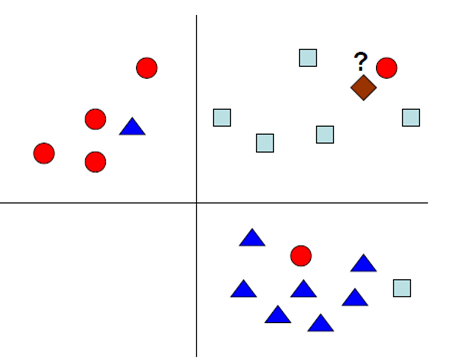
\includegraphics[width=0.6\linewidth]{non_tech_imgs/knn_vis.png}
\end{center}
  \caption{A visualization of the nearest neighbors method.}
  \label{fig:knn_vis}
\end{figure}

\subsection{Configuring the KNN}
Once partitioned the \textit{KNN} effectively makes use of a 10-fold cross-validation for both determining its parameters and performing the general classification. In a total of ten iterations, it trains on nine of the partitions and tests on one. This allows us to predict on ever data point that is available to minimize the opportunity for over-fitting the parameter $k$ and maximizing the validity of the performance results.

\begin{figure}
\begin{center}
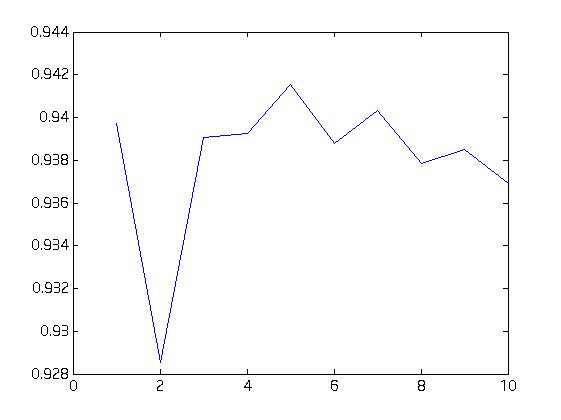
\includegraphics[width=0.6\linewidth]{visual_results/evaluate_k_both_perf.jpg}
\end{center}
\caption{Precision evaluation for number of nearest neighbors.}
\label{fig:eval_k_both_perf}
\end{figure}

\begin{figure}
\begin{center}
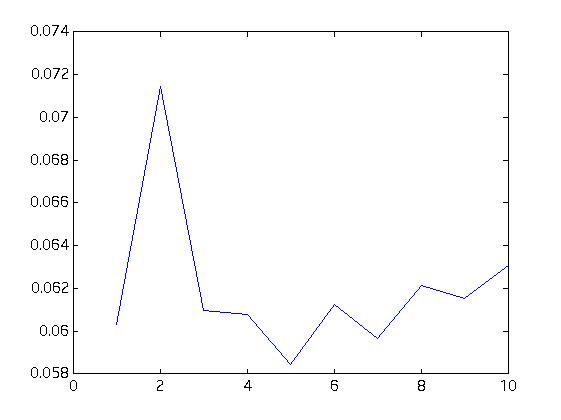
\includegraphics[width=0.6\linewidth]{visual_results/evaluate_k_both_loss_pred_error.jpg}
\end{center}
\caption{Error evaluation for number of nearest neighbors.}
\label{fig:eval_k_both_error}
\end{figure}

Evaluating the number of neighbors is a delicate process where several evaluations is taken into account, seeking a compromise between precision and error. Focusing primarily on minimizing the error rate of the classifier every dataset that was evaluated went through the same parameter validation process. With 11 total different classes the process looked at error and performance for $k$ ranging between one and ten voting neighbors, using a reduced dataset with the same 10-fold cross-validation scheme as in the classification.

The process is illustrated for the combined data set in Figure~\ref{fig:eval_k_both_perf} and Figure~\ref{fig:eval_k_both_error}, visualizing the precision and error rate for $k$ respectively. 

As is usual with this type of deterministic association, $k=1$ nearest neighbor is quite prone to overfitting and even excellent results for this value should be ignored. With quite few classes kind of graph output was typical for all the processed datasets. In this example the optimal number of nearest neighbors is easily observed, as both graphs has their most apparent extremity for $k=5$ which is consequently the optimal $k$ for this dataset of combined data from left and right arm. The results regarding all the datasets processed by the validation scheme is displayed in Table~\ref{tab:optimal_k}.

\begin{table}[bp]
\centering
\caption{Validation results of optimal nearest neighbors.}
\begin{tabular}{|l|l|}
\hline
           			&\textbf{Optimal $k$} 	\\ \hline
\textbf{Left arm}  						& 3 		 				\\ \hline
\textbf{Right arm} 						& 3		 					\\ \hline
\textbf{Combined}  						& 5 						\\ \hline
\textbf{Right arm LDA processed} 		& 7 						\\ \hline
\textbf{Left arm LDA processed} 		& 7 						\\ \hline

\end{tabular}
\label{tab:optimal_k}
\end{table}

%=====================================================================

\section{Analysis}
\subsection{Baseline Classification Performance}
The basis of this study is to first evaluate what the most restrictive classification method can achieve in terms of each activity. The data provided being divided into two separate sets representing respectively the left and right arm the first iteration looks at the performance towards each of these and evaluates the immediate differences.

\subsubsection{Left arm evaluation}


\begin{figure*}
\begin{center}
  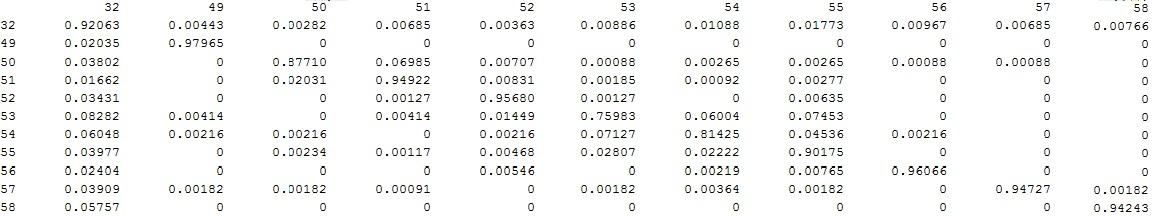
\includegraphics[width=1.0\linewidth]{visual_results/nConfkNN_left.jpg}
\end{center}
  \caption{Confusion matrix for left arm performance.}
  \label{fig:conf_left}
\end{figure*}

\subsubsection{Right arm evaluation}

\begin{figure*}
\begin{center}
  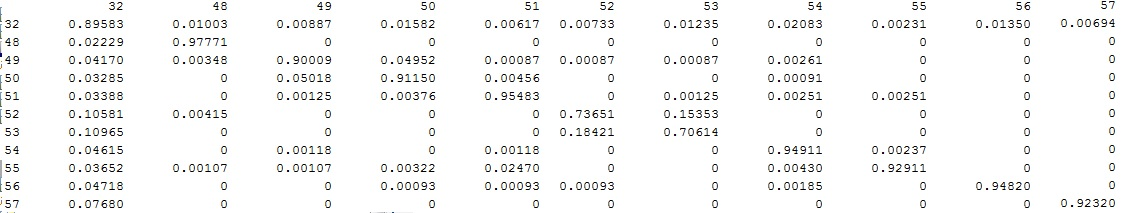
\includegraphics[width=1.0\linewidth]{visual_results/nConfkNN_right.jpg}
\end{center}
  \caption{Confusion matrix for right arm performance.}
  \label{fig:conf_right}
\end{figure*}

\subsubsection{Comparative conclusions}

** Conf mat for each arm 

In a first time we look closer at the baseline performance of our algorithm once applied most elegantly towards a preprocessed version of the original dataset. This approach serves in providing a ground understanding of how well the simplest evaluation of time-series data performs on a very specific set of a limited number of activities once trained on several repetitions of every activity.

** First: Evaluate dataset: Data-set split into right and left with different number of measurements.
- Some activities involves one arm more than the other
- Same sampling rate
- One additional sensor on right arm than left arm: 10\% more data.

** Look at different confusion matrix to evaluate what activities are takes more damage of this - evaluate performance of left and right arm difference by activities performed - which are hurt on each arm and why can that be (opening left door with right arm etc)

** Look at how different activities are recognized by each arm depending on activity -- right arm on left door etc

** Which activities are the baseline already good at - easy to determine by simple classification and feature extraction tools

** Look at $F_1$ score = $2\frac{precision*recall}{precision + recall}$.
While the precision simply represents our classification correctness, the recall rate is bound to the sensitivity of our classifier. Looking at every activity it represents the number of activities classified as a specific activity over the actual sum data points labeled for that activity. The F1 score is widely used to evaluate classification schemes for a compromise between sensitivity and precision.

\subsection{Combining The Data}
The original data provided by \textit{Skoda Mini Checkpoint} does as mentioned contain data separately measured from sensors equally spread and placed on both arms. While it is interesting to evaluate how various activities are recognized with different amounts of success by each arm individually, the study investigates how intelligently merging the two separate datasets improves the recognition. 

This will consequently provide understanding of how more doubling the amount of information or sensors for each measurement increases the general classification performance.

** It makes sense that each activity measure will have begun simultaneously on each arm although one of the arms might have recorded more or less data than the other

** Which activities are immediately easier to determine by combining the data/doubling the sensors - left and right

\begin{figure*}
\begin{center}
  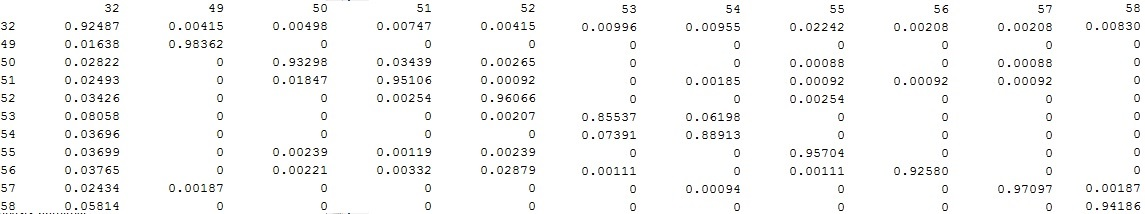
\includegraphics[width=1.0\linewidth]{visual_results/nConfkNN_both.jpg}
\end{center}
  \caption{Confusion matrix for right arm performance.}
  \label{fig:conf_both}
\end{figure*}

\subsection{Feature Selection and Dimensionality Reduction}
When attempting to recognize various activities, different sensors have varying impact on different activities. In collaboration with another team working on the same dataset for \textit{Human Activity Recognition}, the research was enhanced by the possibility of measuring the effect of performing a more extensive feature selection with subsequent dimensionality reduction on the same set of data. 

Looking at the performance of this approach explores the space of improvement in extracting more features while intelligently keeping the ones that should improve the discrimination between the activities and discarding those that make them look more similar.

** Extracting a larger set of features from the time-series data subsequently reduced for optimal classification performance through Linear Discriminant Analysis. LDA efficiently maximizes the mean value of Kullback-Leibler divergence between the activities although assuming Gaussian distribution of the data as well as identical covariance. The technique effectively

** Which activities improves with feature selection

\subsection{Performance Over Different Amounts of Data}
In a real-world application an implemented algorithm should not only perform very accurately, it will optimally also handle real-time received data from the sensors. To approach this with the provided dataset, the study will look at classification performance for percentage amounts of the original data ranging from 10\% to a maximum 100\%.

The original dataset has been assembled sophisticatedly with the aim of satisfying the need for creating a working classification model with a minimum amount of measurements. Through this approach the study analyzes the compromise between classification performance and efficiency with the idea that less data induces higher computational speed.

** What activities need more data to be determined (10\%, 20\%, ..)

%=====================================================================

\section{Results}
Lorem ipsum dolor sit amet, consectetur adipiscing elit. Suspendisse vitae scelerisque enim. Donec venenatis diam eget orci luctus, a semper urna maximus. Fusce tincidunt quam ut mauris consequat, sit amet aliquet sem pharetra. Ut posuere at dolor eu rutrum. Suspendisse tempus ultricies finibus. Nullam dapibus ac diam sed pulvinar. Phasellus convallis felis pretium consectetur interdum. Mauris sagittis nibh sed turpis facilisis dictum. Nam vel risus in mauris fringilla pharetra sed sed turpis. Nunc convallis dolor quam, ut convallis felis viverra quis.

%=====================================================================

\section{Conclusions}

** Which activities are generally more confused

%=====================================================================

\section{Future work}
Lorem ipsum dolor sit amet, consectetur adipiscing elit. Suspendisse vitae scelerisque enim. Donec venenatis diam eget orci luctus, a semper urna maximus. Fusce tincidunt quam ut mauris consequat, sit amet aliquet sem pharetra. Ut posuere at dolor eu rutrum. Suspendisse tempus ultricies finibus. Nullam dapibus ac diam sed pulvinar. Phasellus convallis felis pretium consectetur interdum. Mauris sagittis nibh sed turpis facilisis dictum. Nam vel risus in mauris fringilla pharetra sed sed turpis. Nunc convallis dolor quam, ut convallis felis viverra quis.

%=====================================================================

%\begin{figure}
%\centering
%\epsfig{file=fly.eps}
%\caption{A sample black and white graphic (.eps format).}
%\end{figure}

%\begin{figure}[t]
%\begin{center}
%\fbox{\rule{0pt}{2in}
%   \includegraphics[width=0.3\linewidth]{WorkFlow.png}}
%\end{center}
%   \caption{A workflow diagram of our pipeline.}
%\label{fig:long}
%\label{fig:onecol}
%\end{figure}

% Two columns
%\begin{figure*}
%\centering
%\epsfig{file=flies.eps}
%\caption{A sample black and white graphic (.eps format)
%that needs to span two columns of text.}
%\end{figure*}

% Dual-column table
%\begin{table*}
%\centering
%\caption{Some Typical Commands}
%\begin{tabular}{|c|c|l|} \hline
%Command&A Number&Comments\\ \hline
%\texttt{{\char'134}alignauthor} & 100& Author alignment\\ \hline
%\texttt{{\char'134}numberofauthors}& 200& Author enumeration\\ \hline
%\texttt{{\char'134}table}& 300 & For tables\\ \hline
%\texttt{{\char'134}table*}& 400& For wider tables\\ \hline\end{tabular}
%\end{table*}
% end the environment with {table*}, NOTE not {table}!

%\begin{verbatim}
%{
%    "average_stars": 3.65,
%    "name": "Lene",
%    "review_count": 214,
%    "user_id": "WvhiRlcy-XYwiCof"
%}
%\end{verbatim}

%
% The following two commands are all you need in the
% initial runs of your .tex file to
% produce the bibliography for the citations in your paper.
\bibliographystyle{abbrv}
\bibliography{sigproc}
% add \cite{}'s for bilbiography. fill in sigproc.bib file

\end{document}
